% !TeX encoding = UTF-8
% !TeX program = xelatex
% !TeX spellcheck = en_US

\documentclass[degree=master,language=english]{thuthesis}

% include template setup
% !TeX root = ./main.tex

\thusetup{
  title  = {中文标题(长度不得超过二十五个汉字)},
  title* = {The English Title of Your Capstone Report},
  degree-name  = {管理学硕士},
  degree-name* = {Master of Management Science},
  department = {苏世民书院},
  discipline  = {全球领导力},
  discipline* = {Global Affairs},
  author  = {中文名},
  author* = {You Name},
  % separate the name and title of your supervisor with a common
  supervisor  = {郑纬民, 教授},
  supervisor* = {Professor Zheng Weimin},
  date = {2024-06-18},
  % do not change the options below
  output = electronic,
  include-spine = true,
  toc-depth = 2,
  math-font = xits
}


\usepackage{amsthm}
\usepackage{threeparttable}
\usepackage{multirow}
\usepackage{longtable}
\usepackage{algorithm}
\usepackage{algorithmic}
\usepackage{siunitx}
\usepackage{lipsum}

% do not modify the code below

\graphicspath{{figures/}}

\usepackage[natbibapa]{apacite}
\bibliographystyle{apacite}

\usepackage{hyperref}
\usepackage{schwarzman-extra}


\begin{document}

% 封面 / Title page
\maketitle

% 学位论文指导小组、公开评阅人和答辩委员会名单
% Capstone / Thesis Supervision Committee, Reviewers, and Defense Committee
% !TeX root = ../main.tex

\begin{committee}[name={学位论文公开评阅人和答辩委员会名单}]

  \newcolumntype{C}[1]{@{}>{\centering\arraybackslash}p{#1}}


  \section*{公开评阅人名单}

  \begin{center}
    % \begin{tabular}{C{3cm}C{3cm}C{9cm}@{}}
    无(全匿名评阅)
    % \end{tabular}
  \end{center}


  \section*{答辩委员会名单}

  \begin{center}
    \begin{tabular}{C{2.75cm}C{2.98cm}C{4.63cm}C{4.63cm}@{}}
      主席 & 赵XX                  & 教授                    & 清华大学       \\
      委员 & 刘XX                  & 教授                    & 清华大学       \\
          & \multirow{2}{*}{杨XX} & \multirow{2}{*}{研究员} & 中国XXXX科学院 \\
          &                       &                         & XXXXXXX研究所  \\
          & 黄XX                  & 教授                    & XXXX大学       \\
          & 周XX                  & 副教授                  & XXXX大学       \\
      秘书 & 吴XX                  & 助理研究员              & 清华大学       \\
    \end{tabular}
  \end{center}

\end{committee}



% 也可以导入 Word 版转的 PDF 文件
% \begin{committee}[file=figures/committee.pdf]
% \end{committee}


% 使用授权的说明 / authorization for use
\copyrightpage

% comment out this line for personal capstone report
% !TeX root = ../main.tex

% capstone page
\schcapstone{XXX, YYY, and ZZZ}

% members page
\begin{schmembers}

\begin{center}

\begin{tabular}{|C{0.2\textwidth}|L{0.8\textwidth}|}
\hline
Group Member Name & \multicolumn{1}{c|}{Roles and Responsibilities} \\ \hline
XXX &
\begin{itemize}
\item Responsibility 1
\item Responsibility 2
\end{itemize}
\\ \hline
YYY &
\begin{itemize}
\item Responsibility 3
\item Responsibility 4
\item Responsibility 5
\end{itemize}
\\ \hline
\end{tabular}

\end{center}

\end{schmembers}


\frontmatter

% !TeX root = ../main.tex

% abstracts and keywords

\begin{abstract}
  论文的摘要是对论文研究内容和成果的高度概括。
  摘要应对论文所研究的问题及其研究目的进行描述,对研究方法和过程进行简单介绍,对研究成果和所得结论进行概括。
  摘要应具有独立性和自明性,其内容应包含与论文全文同等量的主要信息。
  使读者即使不阅读全文,通过摘要就能了解论文的总体内容和主要成果。

  论文摘要的书写应力求精确、简明。
  切忌写成对论文书写内容进行提要的形式,尤其要避免“第 1 章……;第 2 章……;……”这种或类似的陈述方式。

  关键词是为了文献标引工作、用以表示全文主要内容信息的单词或术语。
  关键词不超过 5 个,每个关键词中间用分号分隔。

  % 关键词用“英文逗号”分隔,输出时会自动处理为正确的分隔符
  \thusetup{
    keywords = {关键词 , 关键词 , 关键词 , 关键词 , 关键词},
  }
\end{abstract}

\begin{abstract*}
  An abstract of a dissertation is a summary and extraction of research work and contributions.
  Included in an abstract should be description of research topic and research objective, brief introduction to methodology and research process, and summarization of conclusion and contributions of the research.
  An abstract should be characterized by independence and clarity and carry identical information with the dissertation.
  It should be such that the general idea and major contributions of the dissertation are conveyed without reading the dissertation.

  An abstract should be concise and to the point.
  It is a misunderstanding to make an abstract an outline of the dissertation and words “the first chapter”, “the second chapter” and the like should be avoided in the abstract.

  Keywords are terms used in a dissertation for indexing, reflecting core information of the dissertation.
  An abstract may contain a maximum of 5 keywords, with semi-colons used in between to separate one another.

  % Use comma as seperator when inputting
  \thusetup{
    keywords* = {keyword , keyword , keyword , keyword , keyword},
  }
\end{abstract*}


% 目录 / table of contents (auto generated)
\tableofcontents

% 插图和附表清单 / list of figures and tables (optional, auto generated)
\listoffiguresandtables

% 符号对照表 / list of symbols and acronyms (optional)
% !TeX root = ../main.tex

\begin{denotation}[3cm]
  \item[DFT] Density Functional Theory
  \item[HPLC] High Performance Liquid Chromatography
  \item[HPCE] High Performance Capillary Electrophoresis
  \item[IRC] Intrinsic Reaction Coordinates
  \item[LC-MS] Liquid Chromatography-Mass Spectrum
  \item[PES] Potential Energy Surface
  \item[SCF] Self-Consistent Field
  \item[SCRF] Self-Consistent Reaction Field
  \item[TIC] Total Ion Content
  \item[TS] Transition State
  \item[TST] Transition State Theory
  \item[ZPE] Zero Vibration Energy
\end{denotation}


% 正文部分 / main matter
\mainmatter

% include content from data/ folder

% !TeX root = ../main.tex

% modify this file to fill in your content

\chapter{Introduction}

\section{Background}

Tsinghua requires that Chapter 1 be regarded as the Introduction and the final Chapter be regarded as the Conclusion. Consecutively number the pages of your paper, beginning with the Introduction page, throughout the end. Use centered Arabic numerals (1, 2, 3 etc.) at the bottom of each page. Indent the first word of a paragraph 0.74 cm from the left margin, and you can use the tab key of your word-processing program to achieve the indentation (the default setting is likely already 0.74 cm).

Main text …… Figure 1.1 illustrates……

\subsection{Lipsum}

\lipsum[1]

\subsection{Lists}

\begin{itemize}
    \item First, ...
    \item Second, ...
    \begin{enumerate}
        \item Foo, ...
        \item Bar, ...
    \end{enumerate}
\end{itemize}


% !TeX root = ../main.tex

\chapter{Examples of Figures and Tables}

\section{Figures}

Figures are normally inserted in \env{figure} environments by \cs{includegraphics}
You can refer to the source code of Figure~\ref{fig:example}.

It is recommended to use PDF format for vector figures, and JPG format for bitmaps. TIFF format is not supported.

\begin{figure}
  \centering
  
\includegraphics[width=0.6\linewidth]{example-image-a.pdf}
  \caption{Example figure.}
  \label{fig:example}
\end{figure}

If a figure is consisted of two or more sub-figures, the sub-figures should be numbered in (a), (b), (c), etc. and should have sub-captions.

\begin{figure}
  \centering
  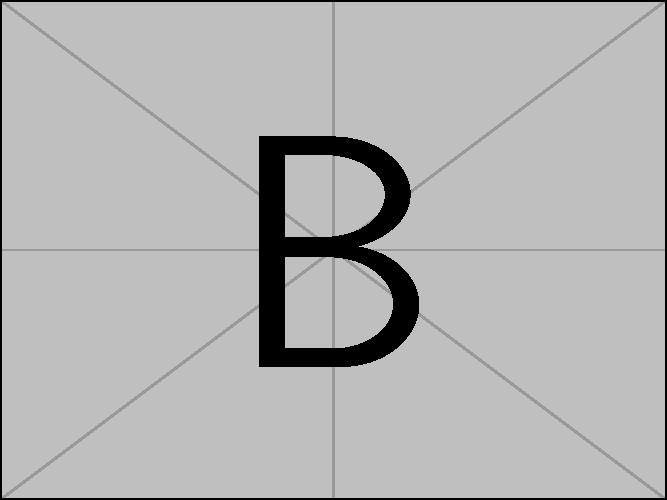
\includegraphics[width=0.6\linewidth]{example-image-b.pdf}
  \caption{Example figure b.}
  \label{fig:example-b}
\end{figure}

It is recommended to use \pkg{subcaption} package to deal with sub-figures, such as Figure~\ref{fig:subfig-a} and Figure~\ref{fig:subfig-b}.

\begin{figure}
  \centering
  \subcaptionbox{Sub-figure A\label{fig:subfig-a}}
    {
\includegraphics[width=0.45\linewidth]{example-image-a.pdf}}
  \subcaptionbox{Sub-figure B\label{fig:subfig-b}}
    {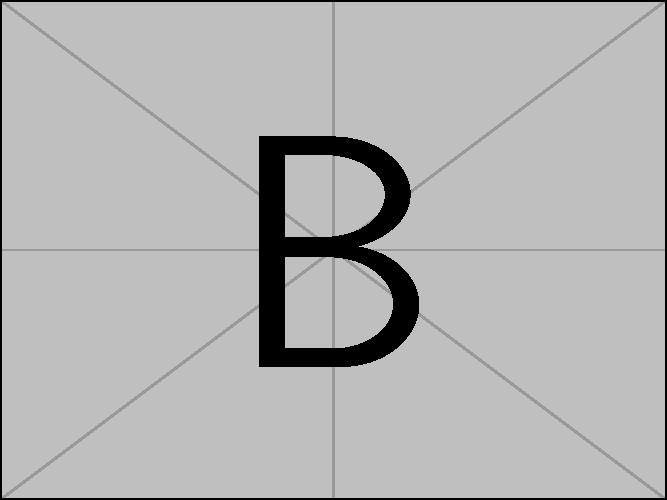
\includegraphics[width=0.45\linewidth]{example-image-b.pdf}}
  \caption{Example figure with two sub-figures.}
  \label{fig:multi-image}
\end{figure}



\section{Tables}

Tables should be self-explanatory. Three line tables are recommended for clearance, such as Table~\ref{tab:three-line}. The three lines can be generated by commands provided by \pkg{booktabs}.

\begin{table}
  \centering
  \caption{Example of a three line table}
  \begin{tabular}{ll}
    \toprule
    Filename          & Description                         \\
    \midrule
    thuthesis.dtx   & 模板的源文件,包括文档和注释 \\
    thuthesis.cls   & 模板文件                     \\
    thuthesis-*.bst & BibTeX 参考文献表样式文件    \\
    thuthesis-*.bbx & BibLaTeX 参考文献表样式文件  \\
    thuthesis-*.cbx & BibLaTeX 引用样式文件        \\
    \bottomrule
  \end{tabular}
  \label{tab:three-line}
\end{table}

If you need to include notes in tables, the package \pkg{threeparttable} can be used.
You must use lower-case letters (a, b, c, ...) to number the notes.

\begin{table}
  \centering
  \begin{threeparttable}[c]
    \caption{Example of a table with notes}
    \label{tab:three-part-table}
    \begin{tabular}{ll}
      \toprule
      Filename                 & Description                         \\
      \midrule
      thuthesis.dtx\tnote{a} & 模板的源文件,包括文档和注释 \\
      thuthesis.cls\tnote{b} & 模板文件                     \\
      thuthesis-*.bst        & BibTeX 参考文献表样式文件    \\
      thuthesis-*.bbx        & BibLaTeX 参考文献表样式文件  \\
      thuthesis-*.cbx        & BibLaTeX 引用样式文件        \\
      \bottomrule
    \end{tabular}
    \begin{tablenotes}
      \item [a] 可以通过 xelatex 编译生成模板的使用说明文档;
        使用 xetex 编译 \file{thuthesis.ins} 时则会从 \file{.dtx} 中去除掉文档和注释,得到精简的 \file{.cls} 文件。
      \item [b] 更新模板时,一定要记得编译生成 \file{.cls} 文件,否则编译论文时载入的依然是旧版的模板。
    \end{tablenotes}
  \end{threeparttable}
\end{table}

The package \pkg{longtable} can be used for cross-page tables.
The number of the table should be repeated on each page, followed by the caption of the table and ``(continued)''. Table heads must also be repeated on continued tables.

\begin{longtable}{cccc}
    \caption{Example of a cross-page long table.} \\
    \toprule
    Column 1 & Column 2 & Column 3 & Column 4 \\
    \midrule
  \endfirsthead
    \caption[]{Example of a cross-page long table (continued).} \\
    \toprule
    Column 1 & Column 2 & Column 3 & Column 4 \\
    \midrule
  \endhead
    \bottomrule
  \endfoot
  Row 1  & & & \\
  Row 2  & & & \\
  Row 3  & & & \\
  Row 4  & & & \\
  Row 5  & & & \\
  Row 6  & & & \\
  Row 7  & & & \\
  Row 8  & & & \\
  Row 9  & & & \\
  Row 10 & & & \\
  Row 11 & & & \\
  Row 12 & & & \\
  Row 13 & & & \\
  Row 14 & & & \\
  Row 15 & & & \\
  Row 16 & & & \\
  Row 17 & & & \\
  Row 18 & & & \\
  Row 19 & & & \\
  Row 20 & & & \\
  Row 21 & & & \\
  Row 22 & & & \\
  Row 23 & & & \\
  Row 24 & & & \\
  Row 25 & & & \\
  Row 26 & & & \\
  Row 27 & & & \\
  Row 28 & & & \\
  Row 29 & & & \\
  Row 30 & & & \\
  Row 31 & & & \\
  Row 32 & & & \\
  Row 33 & & & \\
  Row 34 & & & \\
  Row 35 & & & \\
  Row 36 & & & \\
  Row 37 & & & \\
  Row 38 & & & \\
  Row 39 & & & \\
  Row 40 & & & \\
\end{longtable}


% !TeX root = ../main.tex

\chapter{Maths Symbols and Formulas}

\textbf{This chapter contains Chinese introduction for typesetting formulas in \LaTeX{}. You can safely ignore them and delete the content.}

\makeatletter
\newcommand\dif{%  % 微分符号
  \mathop{}\!%
  \ifthu@math@style@TeX
    d%
  \else
    \mathrm{d}%
  \fi
}
\makeatother

\section{数学符号}

中文论文的数学符号默认遵循 GB/T 3102.11—1993《物理科学和技术中使用的数学符号》
\footnote{原 GB 3102.11—1993,自 2017 年 3 月 23 日起,该标准转为推荐性标准。}。
该标准参照采纳 ISO 31-11:1992 \footnote{目前已更新为 ISO 80000-2:2019。},
但是与 \TeX{} 默认的美国数学学会(AMS)的符号习惯有所区别。
具体地来说主要有以下差异:
\begin{enumerate}
  \item 大写希腊字母默认为斜体,如
    \begin{equation*}
      \Gamma \Delta \Theta \Lambda \Xi \Pi \Sigma \Upsilon \Phi \Psi \Omega.
    \end{equation*}
    注意有限增量符号 $\increment$ 固定使用正体,模板提供了 \cs{increment} 命令。
  \item 小于等于号和大于等于号使用倾斜的字形 $\le$、$\ge$。
  \item 积分号使用正体,比如 $\int$、$\oint$。
  \item 行间公式积分号的上下限位于积分号的上下两端,比如
    \begin{equation*}
      \int_a^b f(x) \dif x.
    \end{equation*}
    行内公式为了版面的美观,统一居右侧,如 $\int_a^b f(x) \dif x$ 。
  \item
    偏微分符号 $\partial$ 使用正体。
  \item
    省略号 \cs{dots} 按照中文的习惯固定居中,比如
    \begin{equation*}
      1, 2, \dots, n \quad 1 + 2 + \dots + n.
    \end{equation*}
  \item
    实部 $\Re$ 和虚部 $\Im$ 的字体使用罗马体。
\end{enumerate}

以上数学符号样式的差异可以在模板中统一设置。
另外国标还有一些与 AMS 不同的符号使用习惯,需要用户在写作时进行处理:
\begin{enumerate}
  \item 数学常数和特殊函数名用正体,如
    \begin{equation*}
      \uppi = 3.14\dots; \quad
      \symup{i}^2 = -1; \quad
      \symup{e} = \lim_{n \to \infty} \left( 1 + \frac{1}{n} \right)^n.
    \end{equation*}
  \item 微分号使用正体,比如 $\dif y / \dif x$。
  \item 向量、矩阵和张量用粗斜体(\cs{symbf}),如 $\symbf{x}$、$\symbf{\Sigma}$、$\symbfsf{T}$。
  \item 自然对数用 $\ln x$ 不用 $\log x$。
\end{enumerate}


英文论文的数学符号使用 \TeX{} 默认的样式。
如果有必要,也可以通过设置 \verb|math-style| 选择数学符号样式。

关于量和单位推荐使用
\href{http://mirrors.ctan.org/macros/latex/contrib/siunitx/siunitx.pdf}{\pkg{siunitx}}
宏包,
可以方便地处理希腊字母以及数字与单位之间的空白,
比如:
\SI{6.4e6}{m},
\SI{9}{\micro\meter},
\si{kg.m.s^{-1}},
\SIrange{10}{20}{\degreeCelsius}。



\section{数学公式}

数学公式可以使用 \env{equation} 和 \env{equation*} 环境。
注意数学公式的引用应前后带括号,建议使用 \cs{eqref} 命令,比如式 \eqref{eq:example}。
\begin{equation}
  \frac{1}{2 \uppi \symup{i}} \int_\gamma f = \sum_{k=1}^m n(\gamma; a_k) \mathscr{R}(f; a_k)
  \label{eq:example}
\end{equation}
注意公式编号的引用应含有圆括号,可以使用 \cs{eqref} 命令。

多行公式尽可能在“=”处对齐,推荐使用 \env{align} 环境。
\begin{align}
  a & = b + c + d + e \\
    & = f + g
\end{align}



\section{数学定理}

定理环境的格式可以使用 \pkg{amsthm} 或者 \pkg{ntheorem} 宏包配置。
用户在导言区载入这两者之一后,模板会自动配置 \env{thoerem}、\env{proof} 等环境。

\begin{theorem}[Lindeberg--Lévy 中心极限定理]
  设随机变量 $X_1, X_2, \dots, X_n$ 独立同分布, 且具有期望 $\mu$ 和有限的方差 $\sigma^2 \ne 0$,
  记 $\bar{X}_n = \frac{1}{n} \sum_{i+1}^n X_i$,则
  \begin{equation}
    \lim_{n \to \infty} P \left(\frac{\sqrt{n} \left( \bar{X}_n - \mu \right)}{\sigma} \le z \right) = \Phi(z),
  \end{equation}
  其中 $\Phi(z)$ 是标准正态分布的分布函数。
\end{theorem}
\begin{proof}
  Trivial.
\end{proof}

同时模板还提供了 \env{assumption}、\env{definition}、\env{proposition}、
\env{lemma}、\env{theorem}、\env{axiom}、\env{corollary}、\env{exercise}、
\env{example}、\env{remar}、\env{problem}、\env{conjecture} 这些相关的环境。


% !TeX root = ../main.tex

\chapter{Citations and References}

\section{Citations}

Parenthetical citation: \citep{mellinger1996laser} said ...

Text citation: \citet{dupont1974bone} proposed ...

You should add more items in \texttt{ref/refs.bib} and cite them in your text.


% add more files ...
% \input{data/chap05}

% 其他部分 / back matter
\backmatter

% 参考文献 / references (auto generated from citations in text)
\bibliography{ref/refs}

% 附录 / appendices
\appendix

% !TeX root = ../main.tex

\chapter{Auxiliary Content}


\section{Examples of figures and tables}

\subsection{Figures}

Example of a figure in appendix (Figure~\ref{fig:appendix-figure}).

\begin{figure}
  \centering
  
\includegraphics[width=0.6\linewidth]{example-image-a.pdf}
  \caption{Example of a figure in appendix}
  \label{fig:appendix-figure}
\end{figure}


\subsection{Tables}

Example of a table in appendix (Table~\ref{tab:appendix-table}).

\begin{table}
  \centering
  \caption{Example of a table in appendix}
  \begin{tabular}{ll}
    \toprule
    Filename          & Description                         \\
    \midrule
    thuthesis.dtx   & 模板的源文件,包括文档和注释 \\
    thuthesis.cls   & 模板文件                     \\
    thuthesis-*.bst & BibTeX 参考文献表样式文件    \\
    thuthesis-*.bbx & BibLaTeX 参考文献表样式文件  \\
    thuthesis-*.cbx & BibLaTeX 引用样式文件        \\
    \bottomrule
  \end{tabular}
  \label{tab:appendix-table}
\end{table}


\section{Formulas}

Example of a formula in appendix (Equation~\eqref{eq:appendix-equation}).

\begin{equation}
  \frac{1}{2 \uppi \symup{i}} \int_\gamma f = \sum_{k=1}^m n(\gamma; a_k) \mathscr{R}(f; a_k)
  \label{eq:appendix-equation}
\end{equation}


% 致谢 / acknowledges
% !TeX root = ../main.tex

\begin{acknowledgements}
  I would like to express my gratitude towards...
\end{acknowledgements}


% 声明 / statements
\statement

% 个人简历、在学期间完成的相关学术成果 / resume
% !TeX root = ../main.tex

\begin{resume}

Your Name was born on 22nd November 1990 in City, Province/State, Country.

She/He began her/his bachelor’s study in the School/Department of XXX, XXX University in September 2008, majoring in physics, and got a Bachelor of Science degree in July 2012.

She/He began her/his master’s study in the School/Department of XXX, XXX University in September 2012, and got a Master of Science degree in Physics in July 2014.

She/He has started to pursue a doctor’s degree in Physics in the School/Department of XXX, Tsinghua University since September 2014. During this period, she/he has made academic achievements as follows.

  \subsection*{Monograph}
  \begin{achievements}
    \item Yang Y, Ren T L, Zhang L T, et al. Miniature microphone with silicon-based ferroelectric thin films[J]. Integrated Ferroelectrics, 2003, 52:229-235.
  \end{achievements}

  \subsection*{Journal article}
  \begin{achievements}
    \item 杨轶, 张宁欣, 任天令, 等. 硅基铁电微声学器件中薄膜残余应力的研究[J]. 中国机械工程, 2005, 16(14):1289-1291.
    \item 杨轶, 张宁欣, 任天令, 等. 集成铁电器件中的关键工艺研究[J]. 仪器仪表学报, 2003, 24(S4):192-193.
    \item Yang Y, Ren T L, Zhu Y P, et al. PMUTs for handwriting recognition. In press[J]. (已被Integrated Ferroelectrics录用)
  \end{achievements}


  \subsection*{Patent}
  \begin{achievements}
    \item 任天令, 杨轶, 朱一平, 等. 硅基铁电微声学传感器畴极化区域控制和电极连接的方法: 中国, CN1602118A[P]. 2005-03-30.
    \item Ren T L, Yang Y, Zhu Y P, et al. Piezoelectric micro acoustic sensor based on ferroelectric materials: USA, No.11/215, 102[P]. (美国发明专利申请号.)
  \end{achievements}

\end{resume}


% 指导教师/指导小组学术评语 / comments from thesis supervisor
% !TeX root = ../main.tex

\begin{comments}
% \begin{comments}[name = {指导小组学术评语}]
% \begin{comments}[name = {Comments from Thesis Supervisor}]
% \begin{comments}[name = {Comments from Thesis Supervision Committee}]

The thesis proposes...

\end{comments}


% 答辩委员会决议书 / resolution of thesis defense committee
% !TeX root = ../main.tex

\begin{resolution}

  The thesis proposes...
  
  The main novelty of the thesis is ...

  答辩委员会表决,(×票/一致)同意通过论文答辩,并建议授予×××(姓名)×××(门类)学博士/硕士学位。

\end{resolution}


\end{document}
